\chapter{ Results }
\label{results}


\section{Simulation outputs - RL Circuit}


In order to demonstrate that the results obtained by the Haskell ETR-P version are the same as the ones in the Matlab version, a simulation using the same parameters in both Matlab and Haskell version is adopted. The chosen circuit configuration, components and simulation values are presented at \cref{lst:csv1r} and at \cref{lst:csv2r} (which happen to be the same values used at \cref{implhs}). The circuit is shown in \cref{thesissim1}.

\begin{figure}[H]
   \centering
   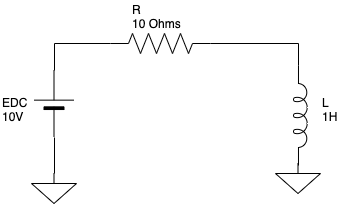
\includegraphics[width=0.7\textwidth]{img/thesissim1.png}
   \caption{DC Circuit}
   \label{thesissim1}
\end{figure}

\begin{lstlisting}[language=bash, label=getinfo, caption={Input data file for components in the Haskell implementation}, captionpos=b, label={lst:csv1r}]
Element Type,Node K,Node M,Value,Source param 1,Source param 2,Plot
EDC,2,0,10,0,0,0 
R,2,1,10,0,0,0
L,1,0,1,0,0,0
\end{lstlisting}


\begin{lstlisting}[language=bash, label=getinfo, caption={Input data file for time}, captionpos=b, label={lst:csv2r}]
Number of Nodes,Number of Voltages Sources,Step Size,Maximum time for simulation
2,1,0.0001,0.0005
\end{lstlisting}

The same setup in ETR-P is given by the file shown at \cref{lst:inputthtar}.

\begin{lstlisting}[language=bash, label=getinfo, caption={Original input data file for ETR-P Matlab}, captionpos=b, label={lst:inputthtar}]
T   2   1   100E-6  5E-4    0   0   0   0   0
EDC 2   0   10      0       0   0   0   0   5
R   2   1   10      0       0   0   0   0   5
L   1   0   1       0       0   0   0   0   5
NV  1   2   0       0       0   0   0   0   0
\end{lstlisting}


\subsection{ Short simulation with DC Voltage}

The simulation time is only 0.0005 seconds, which gives us only 6 \lstinline!npoints! for the step size of 0.0001. In a later section of this chapter, a longer simulation will be tested and executed.

In the Matlab version, it is possible to log the results from each iteration step by removing the semi-colons at the end of each line, or by explicitly calling the command \lstinline!fprintf!, as the example in \cref{lst:logthtar}.

\begin{lstlisting}[language=Matlab, label=getinfo, caption={Logging the results of V and I at the end of each iteration in Matlab}, captionpos=b, label={lst:logthtar}]
%% Build vector IA for the time t
    IA = I(1:D, 1);
    
    %% Build the vector RHSA for the time t
    RHSA = IA - GAB*VB;
    
    %% Solve for vector VA at the time t
    VA = GAA\RHSA;
    IB = GBA*VA+GBB*VB;
    I = [IA; IB];
    %% Build vector V at the time t (i.e.,  time counter or point n)
    V(:, n) = [VA; VB];
    
    fprintf('---------------- I final in every step of the loop -----------\n');
    I
    fprintf('---------------- V final in every step of the loop -----------\n');
    V
\end{lstlisting}

Logging and debugging is not equally straightforward in Haskell. A log would represent an impurity, since it writes at the standard output. To print out the values of operations in pure functions, it is necessary to use the \lstinline!Debug.Trace! library. To log the values of \lstinline!I! and \lstinline!V! in every iteration, there must be a call to the \lstinline!Trace.trace! function in some of the let binding in the \lstinline!thtaSimulationStep! function. Example in \cref{lst:logginghs}.

\begin{lstlisting}[language=Haskell, numbers=left, caption={Logging the values of I and V at the Haskell implementation}, captionpos=b, label={lst:logginghs}]
thtaSimulationStep :: [ComponentData] -> Matrix Double -> [Double] -> SimulationData -> Int -> Int -> Double  -> Vector Double -> Matrix Double -> Vector Double -> Vector Double -> SimulationResults
thtaSimulationStep _ _ _ _ _ 1 _ _ vMatrix _ iVector = (iVector, vMatrix)
thtaSimulationStep components condutances gkms simulation thtactl n time ih vMatrix vbVector iVector =
  let (gaa, gab, gba, gbb) = Matrix.splitBlocks ((nodes simulation) - (voltageSources simulation)) ((nodes simulation) - (voltageSources simulation)) condutances
      ihBuffer = buildIhVector components gkms n ih (Vector.replicate (nh (Vector.fromList components)) 0) vMatrix
      vbVec = buildVBVector components
      (thta, ihThta, timeThta) = thtaControl thtactl time ihBuffer ih
      iVec = buildIVector components ihThta (Vector.replicate (nodes simulation) 0)
      (iVecCalc, vVec) = Trace.trace ("Solver = \n" ++ show (solver (toHMatrixVectorTransformer iVec) (toHMatrixTransformer gaa) (toHMatrixTransformer gab) (toHMatrixTransformer gba) (toHMatrixTransformer gbb) (toHMatrixVectorTransformer vbVec) simulation)) solver (toHMatrixVectorTransformer iVec) (toHMatrixTransformer gaa) (toHMatrixTransformer gab) (toHMatrixTransformer gba) (toHMatrixTransformer gbb) (toHMatrixVectorTransformer vbVec) simulation
      vMatr = Trace.trace ("vMatrix = \n" ++ show (Matrix.mapCol (\r _ -> vVec Vector.! (r - 1)) (n-1) vMatrix)) Matrix.mapCol (\r _ -> vVec Vector.! (r - 1)) (n-1) vMatrix
  in
      thtaSimulationStep components condutances gkms simulation thta (n-1) time ihThta vMatr vbVec iVecCalc

\end{lstlisting}

\subsubsection{Step 0}
Initial step. Everything is set to 0.0.

\subsubsection{Step 1}

Results in Haskell - \cref{h1}:

\begin{figure}[H]
   \centering
   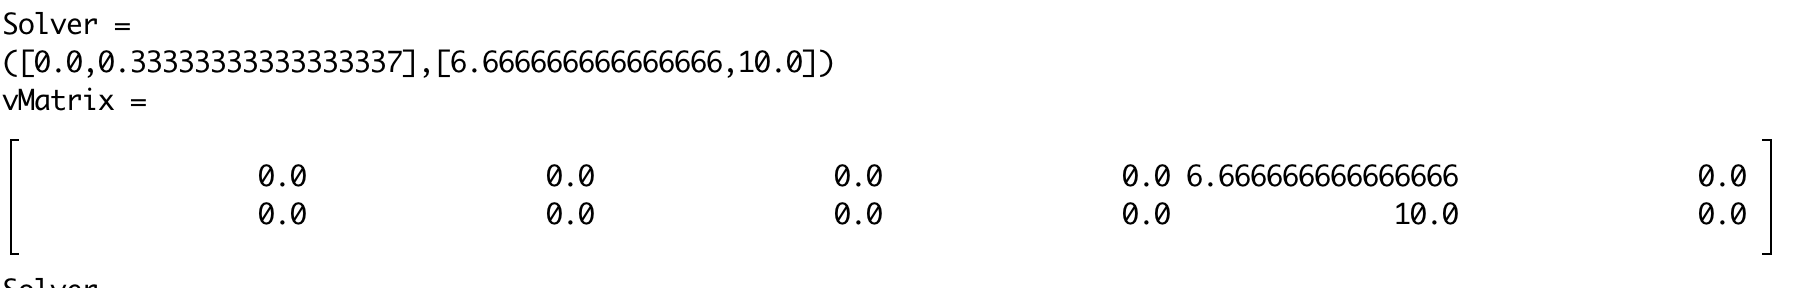
\includegraphics[width=0.9\textwidth]{img/h1.png}
   \caption{Results for step 5 - Haskell (recall that the Haskell loop stars from the highest value of the iteration, which is 5)}
   \label{h1}
\end{figure}

Results form Matlab - \cref{m1}:

\begin{figure}[H]
   \centering
   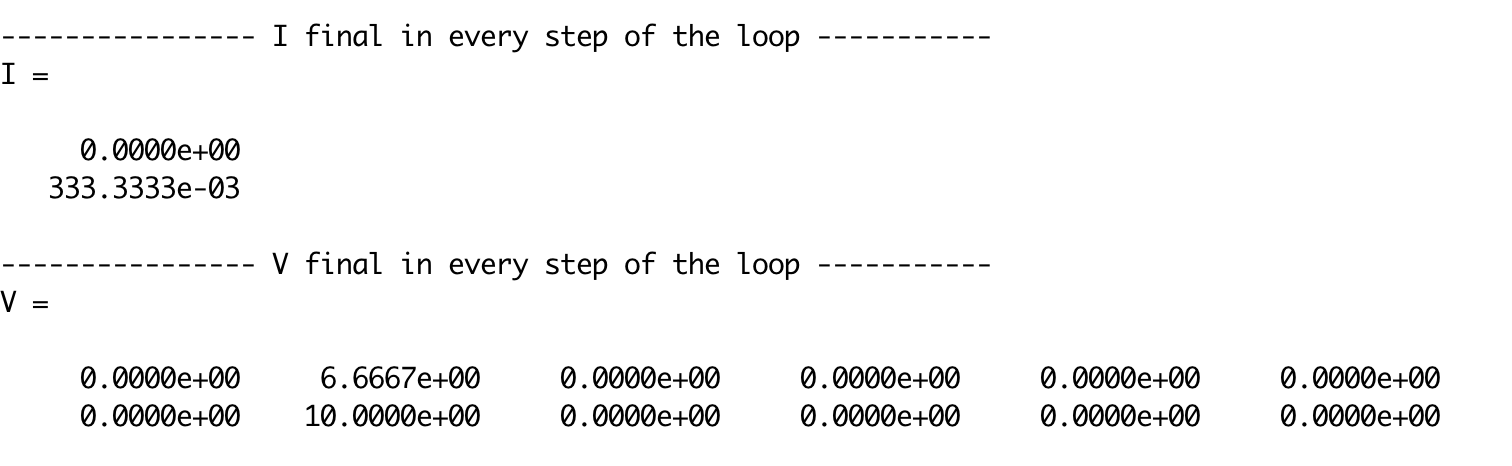
\includegraphics[width=0.9\textwidth]{img/m1.png}
   \caption{Results for step 1 - Matlab}
   \label{m1}
\end{figure}


\subsubsection{Step 2}

Results in Haskell - \cref{h2}:

\begin{figure}[H]
   \centering
   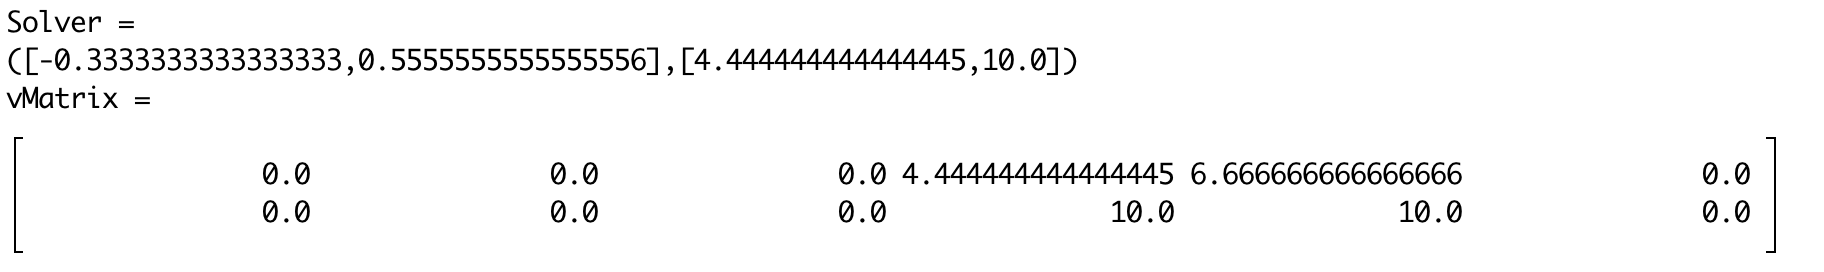
\includegraphics[width=0.9\textwidth]{img/h2.png}
   \caption{Results for step 4 - Haskell}
   \label{h2}
\end{figure}

Results form Matlab - \cref{m2}:

\begin{figure}[H]
   \centering
   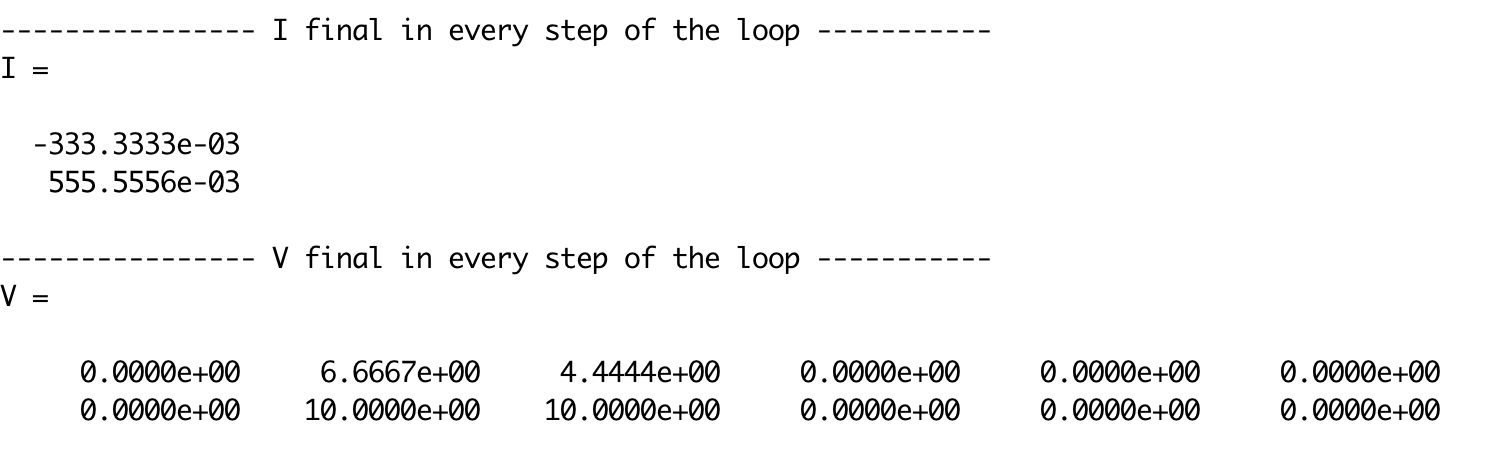
\includegraphics[width=0.9\textwidth]{img/m2.png}
   \caption{Results for step 2 - Matlab}
   \label{m2}
\end{figure}


\subsubsection{Step 3}

Results in Haskell - \cref{h3}:

\begin{figure}[H]
   \centering
   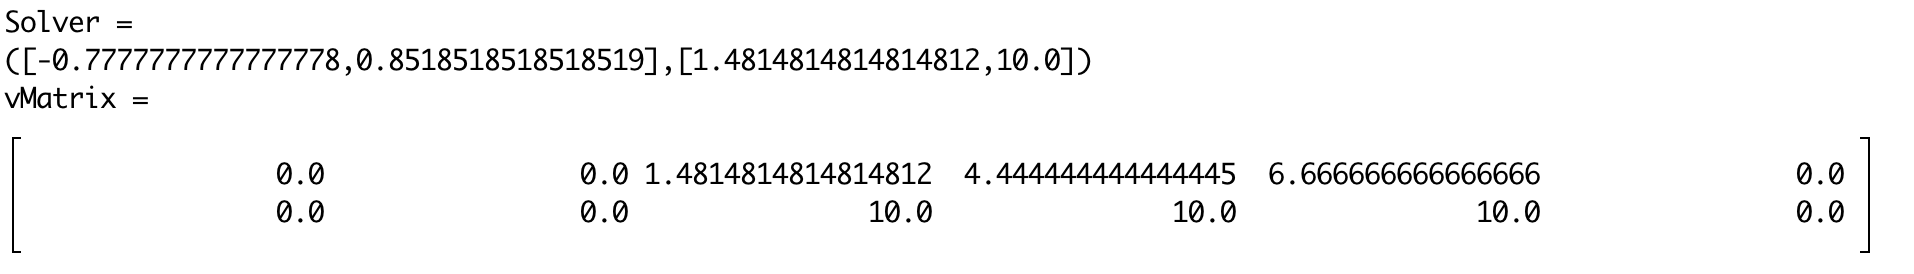
\includegraphics[width=0.9\textwidth]{img/h3.png}
   \caption{Results for step 3 - Haskell}
   \label{h3}
\end{figure}

Results form Matlab - \cref{m3}:

\begin{figure}[H]
   \centering
   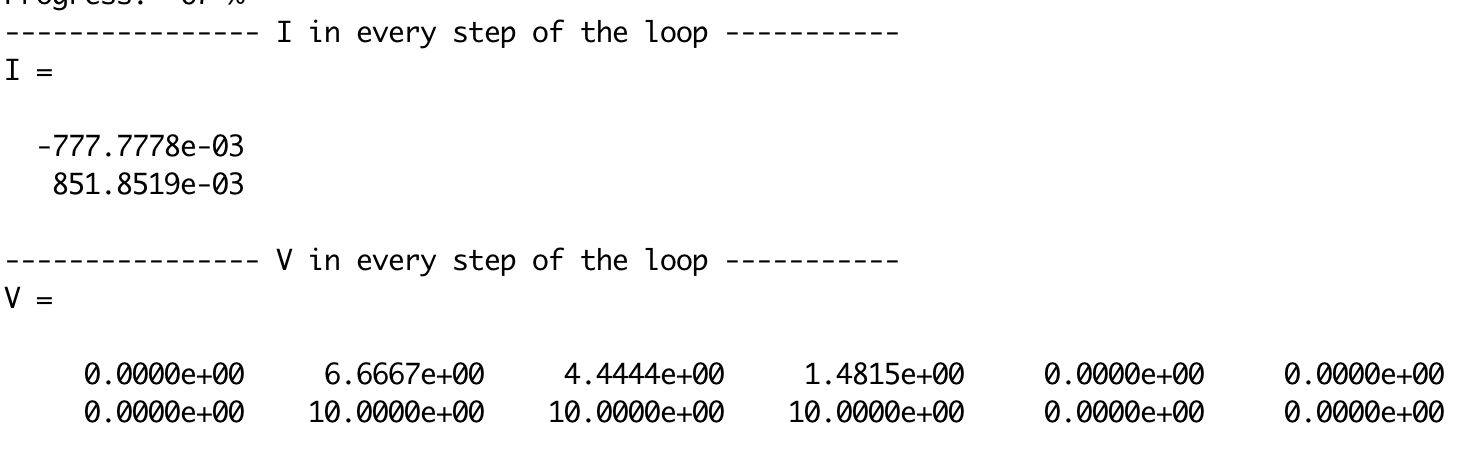
\includegraphics[width=0.9\textwidth]{img/m3.png}
   \caption{Results for step 3 - Matlab}
   \label{m3}
\end{figure}


\subsubsection{Step 4}

Results in Haskell - \cref{h5}:

\begin{figure}[H]
   \centering
   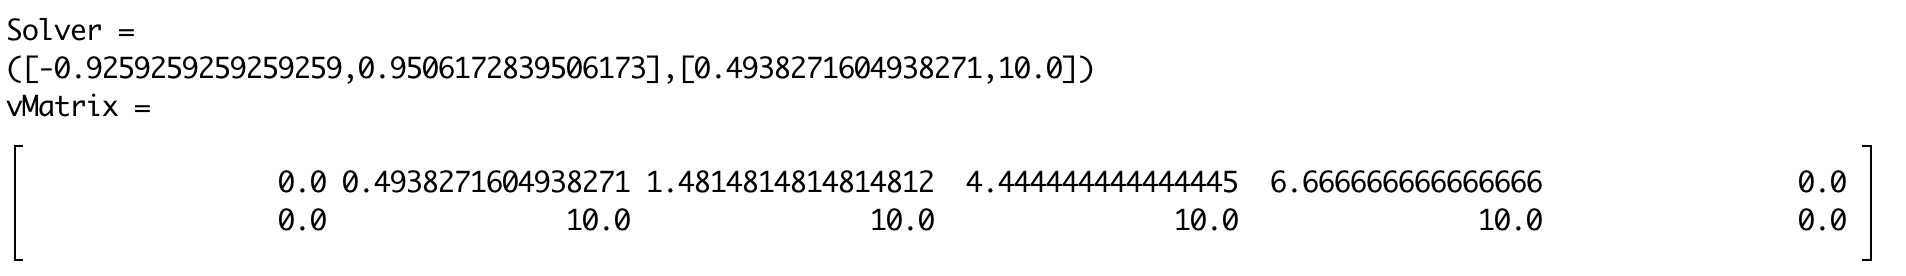
\includegraphics[width=0.9\textwidth]{img/h5.png}
   \caption{Results for step 2 - Haskell}
   \label{h5}
\end{figure}

Results form Matlab - \cref{m5}:

\begin{figure}[H]
   \centering
   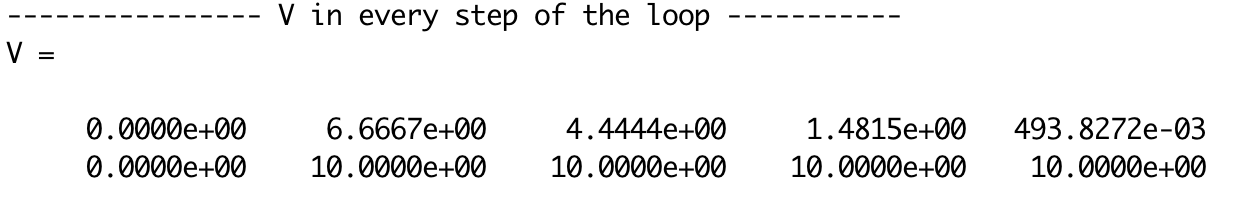
\includegraphics[width=0.7\textwidth]{img/m5.png}
   \caption{Results for step 4 - Matlab}
   \label{m5}
\end{figure}


\subsubsection{Step 5 - final step}


Figure \ref{reschart1} is a plot of both simulations for the voltage outputs of the V Matrix. There are no significant differences between the results and the curves are on the same place.


\begin{figure}[H]
   \centering
   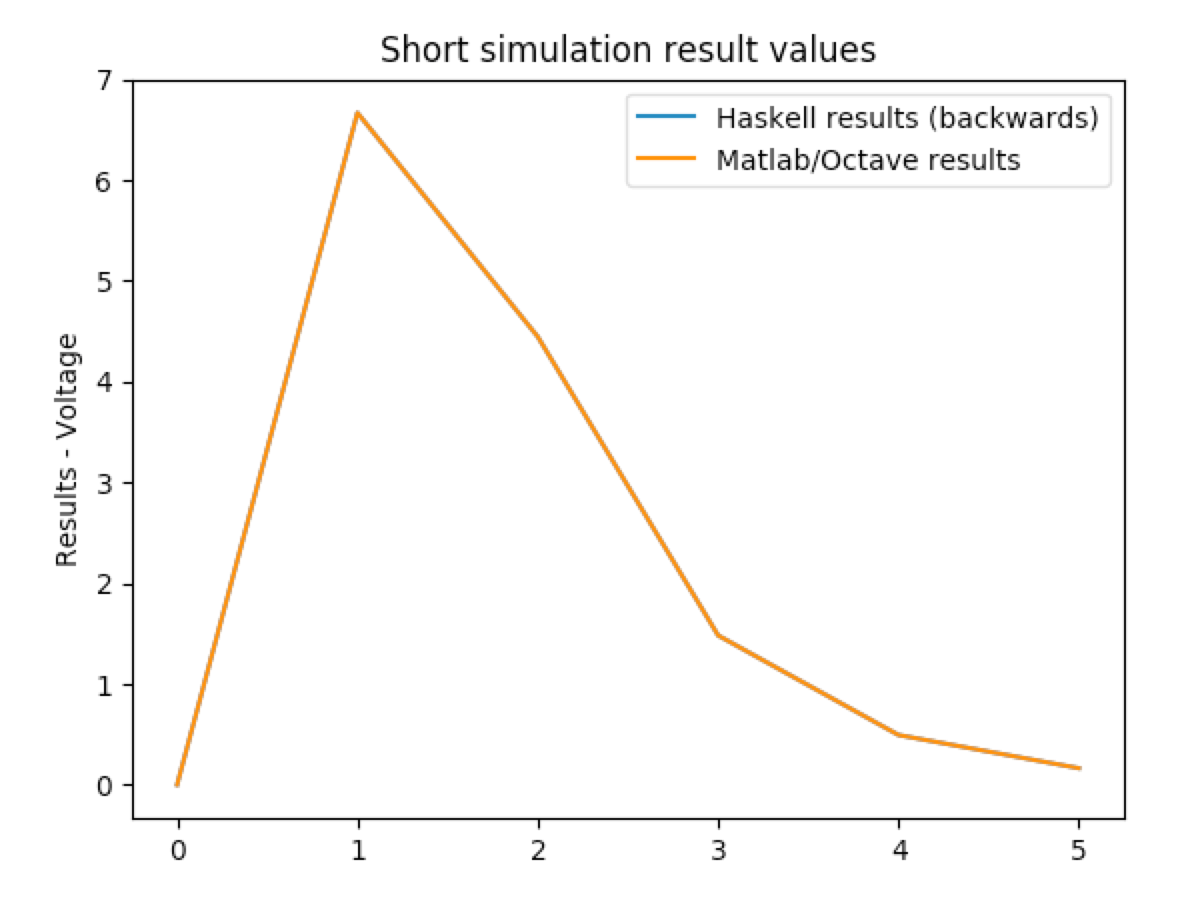
\includegraphics[width=0.7\textwidth]{img/voltageplot.png}
   \caption{Short simulation results chart - V}
   \label{reschart1}
\end{figure}

Figure \ref{iachart} and \cref{ibchart} are the chars for IA and IB results, respectively:

\begin{figure}[H]
   \centering
   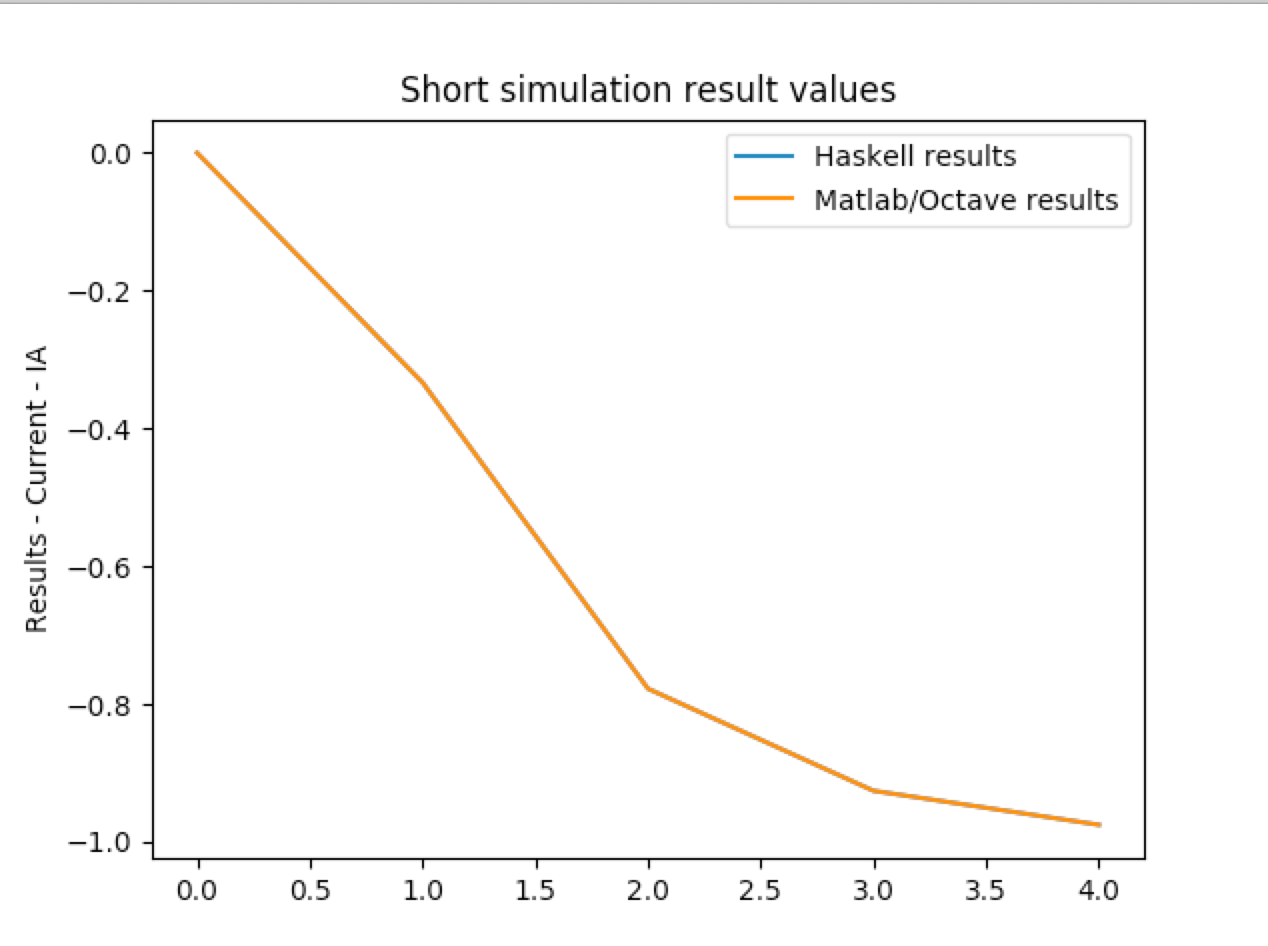
\includegraphics[width=0.7\textwidth]{img/iaplot.png}
   \caption{Short simulation results chart - IA}
   \label{iachart}
\end{figure}



\begin{figure}[H]
   \centering
   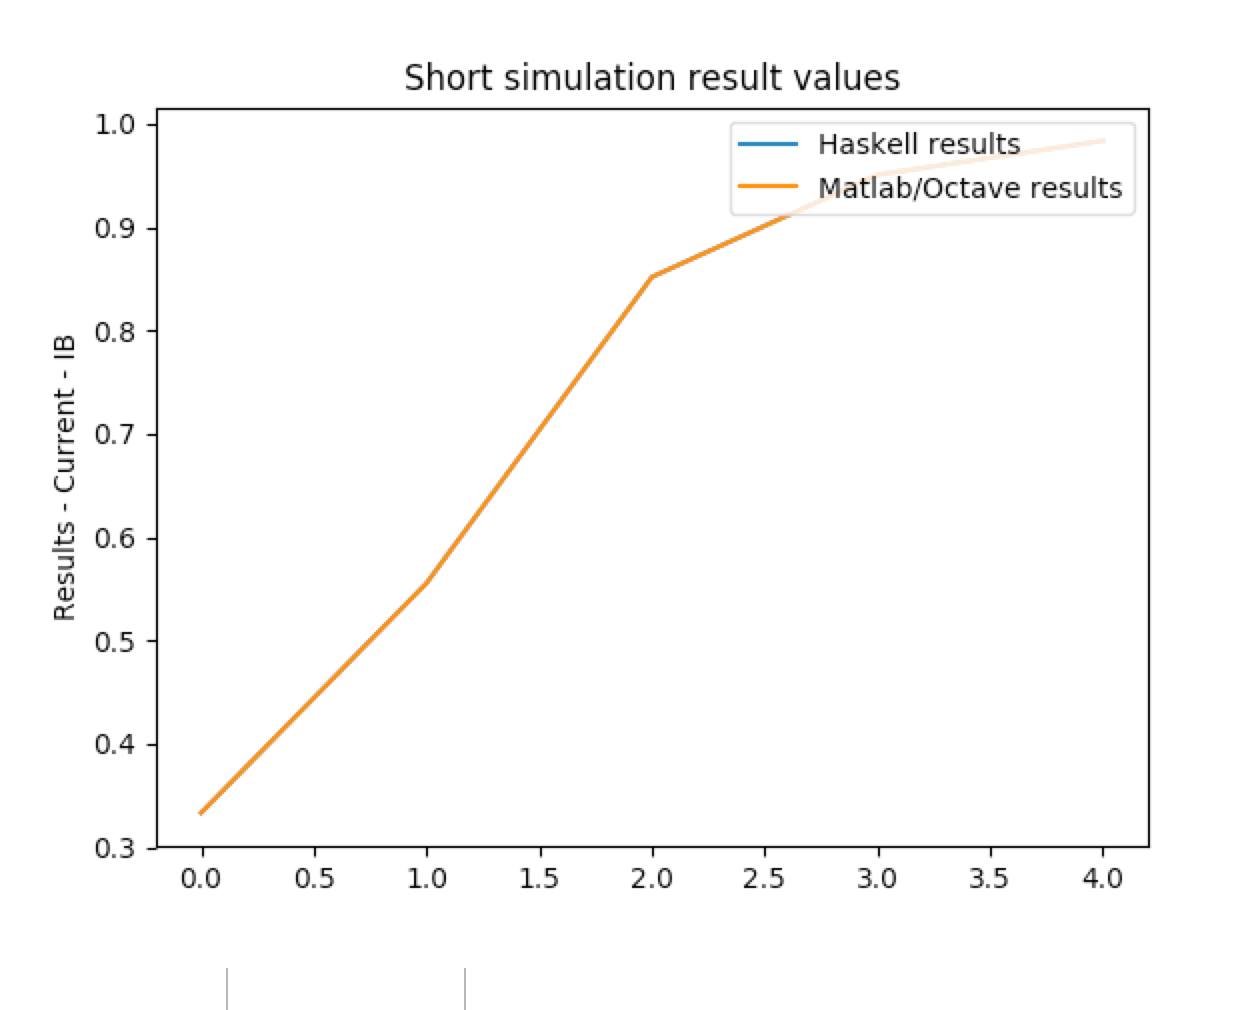
\includegraphics[width=0.9\textwidth]{img/ibplot.png}
   \caption{Short simulation results chart - IB}
   \label{ibchart}
\end{figure}

Note: The charts were plotted using Python to avoid bias towards the two languages during the comparison process.

The final V Matrix is described in \cref{tab:hsresults}.

% Please add the following required packages to your document preamble:
% \usepackage{graphicx}
\begin{table}[H]
\resizebox{\textwidth}{!}{%
\begin{tabular}{llllll}
Step 5              & Step 4             & Step 3             & Step 2            & Step 1            & Step 0 \\
0.16460905349794236 & 0.4938271604938271 & 1.4814814814814812 & 4.444444444444445 & 6.666666666666666 & 0.0    \\
10.0                & 10.0               & 10.0               & 10.0              & 10.0              & 0.0   
\end{tabular}%
}
\caption{V Matrix calculated for the Haskell implementation. The results go from right to left. Each column represents one step of the iteration}
\label{tab:hsresults}
\end{table}

The final V Matrix from the Matlab implementation is listed in \cref{tab:thtamatlabv}.

% Please add the following required packages to your document preamble:
% \usepackage{graphicx}
\begin{table}[H]
\resizebox{\textwidth}{!}{%
\begin{tabular}{llllll}
Step 0     & Step 1      & Step 2      & Step 3      & Step 4       & Step 5      \\
0.0000e+00 & 6.6667e+00  & 4.4444e+00  & 1.4815e+00  & 493.8272e-03 & 164.6091e-03 \\
0.0000e+00 & 10.0000e+00 & 10.0000e+00 & 10.0000e+00 & 10.0000e+00  & 10.0000e+00
\end{tabular}%
}
\caption{V Matrix calculated for the Matlab implementation. The results go from left to right.}
\label{tab:thtamatlabv}
\end{table}

It is important to also compare the results from the \lstinline!I! Vector. For the Haskell implementation, the final values are $ [-0.9753086419753086,0.9835390946502057] $ and for the Matlab ETR-P, the values are $ [-975.3086e-03, 983.5391e-03] $. As expected, those are very close values (numerically).


\subsection{ Long simulation with DC Voltage }
\label{longsimmm}

With some initial guarantees of a successful short simulation, it becomes reasonable to run a longer simulation (setting up \lstinline!tmax! for 0.05) and then compare the results. 

When analysing the final \lstinline!V! Matrices of this longer simulation, it is possible to notice they will be both square and triangular matrices. Several values will be either 0.0 or 10.0 (EDC Voltage source). The transient, calculated values are compared in \ref{fig:haskellvmatrfinal}.

\begin{figure}[H]
   \centering
   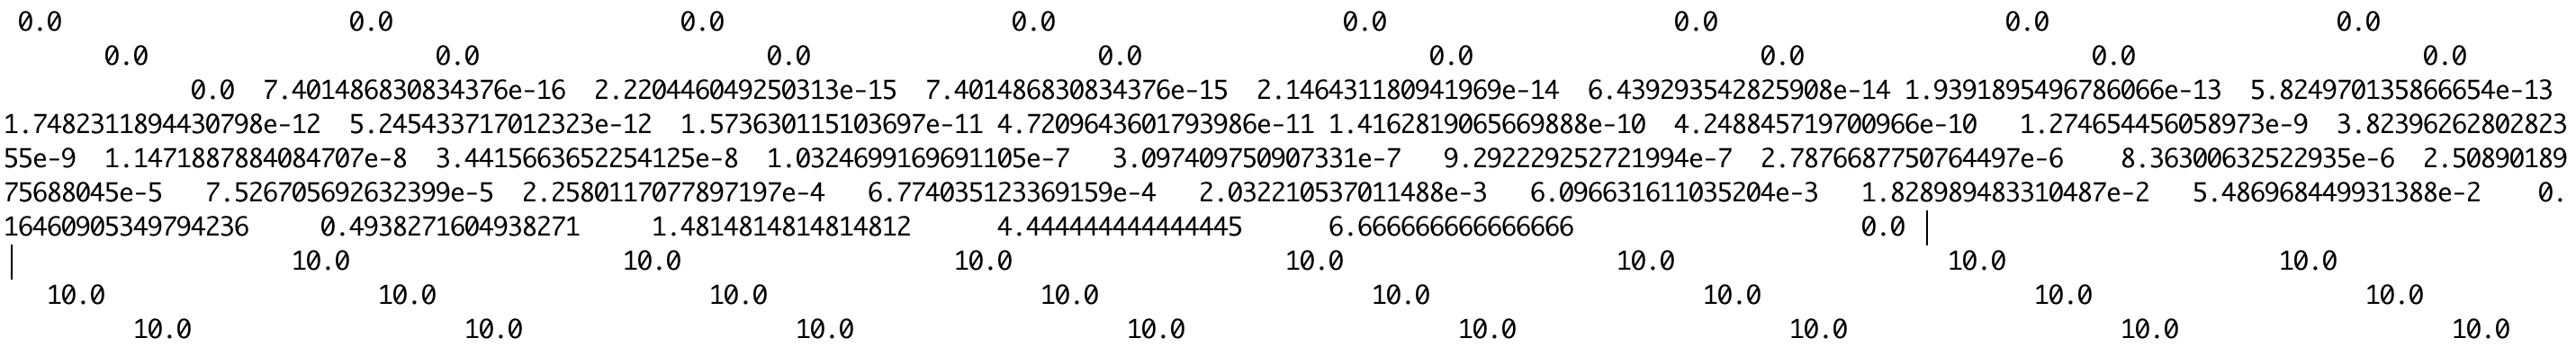
\includegraphics[width=0.9\textwidth]{img/results_Haskell.png}
   \caption{Results for the triangular Matrix V in a broader simulation with Haskell}
   \label{fig:haskellvmatrfinal}
\end{figure}


\begin{figure}[H]
   \centering
   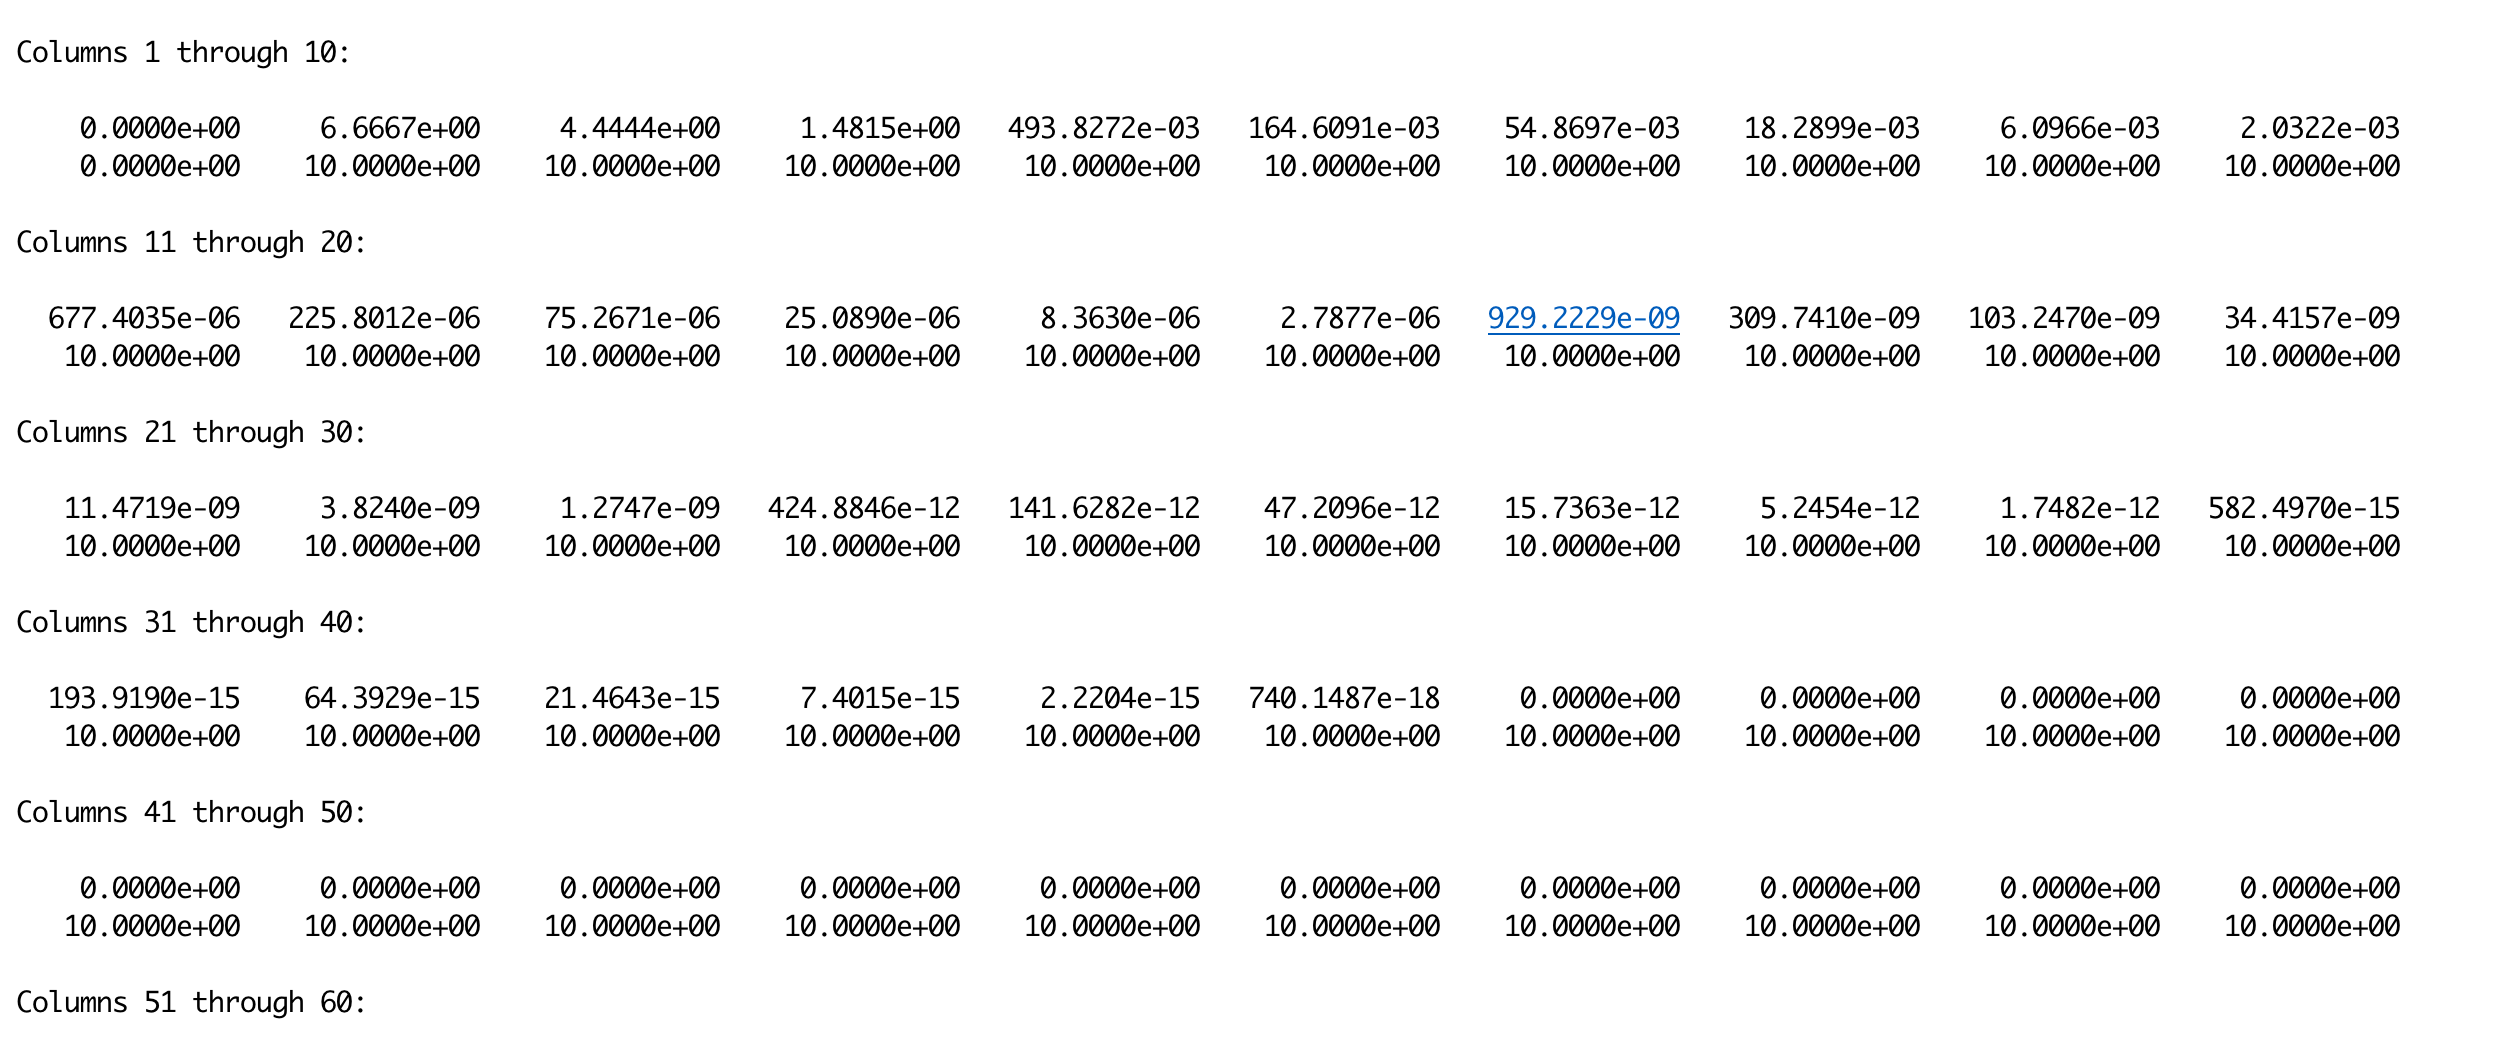
\includegraphics[width=0.9\textwidth]{img/results_THTA_Matlab.png}
   \caption{Results for the triangular Matrix V in a broader simulation with THTA Matlab}
   \label{matlabvmatrfinal}
\end{figure}

Compare the first value of the figure \ref{fig:haskellvmatrfinal} (7.401486830834376e-16) with the last result which is not 0 at \ref{matlabvmatrfinal}. By contrasting first and last pairs, it is possible to notice the values are very similar (numerically). It is then demonstrated that the program works as expected according to the ETR-P algorithm.


Figure \ref{reschart2} is a plot of both simulations for the voltage outputs of the V Matrix in this longer simulation. There are no significant differences between the results. Only the transient values appear in this plot to allow the value comparison.


\begin{figure}[H]
   \centering
   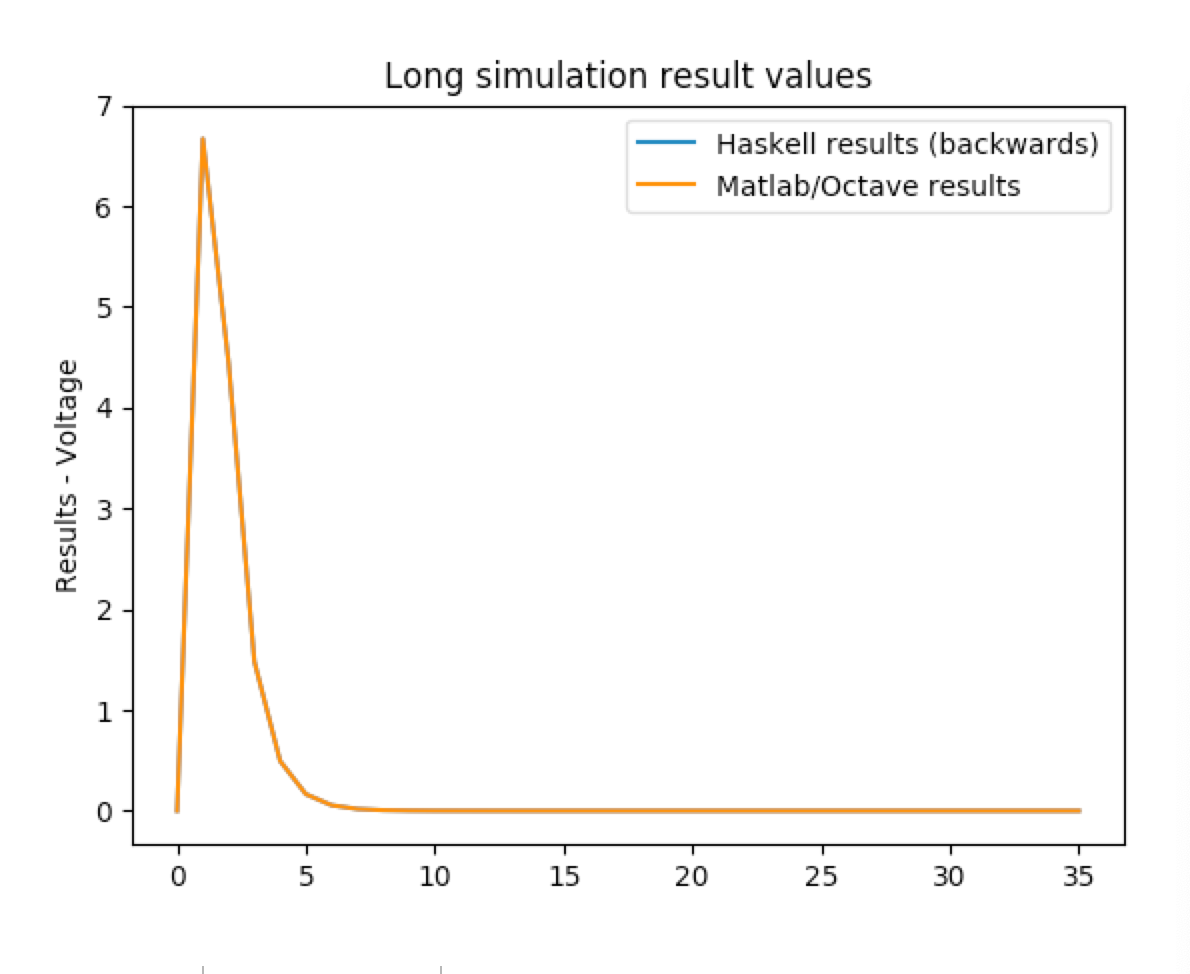
\includegraphics[width=0.7\textwidth]{img/voltageplotlong.png}
   \caption{Long simulation results chart - V}
   \label{reschart2}
\end{figure}

Note: The chart was plotted using Python to avoid bias towards the two languages during the comparison process.

Once again the results are pretty accurate and result in two overlapping curves.

Next, \cref{fig:dcresultsmicro} and \cref{fig:dcresultsmicrooctave} shows the results for the voltage outputs when setting up \lstinline!tmax! for 0.01s and the step size of 0.000001s.

\begin{figure}[H]
   \centering
   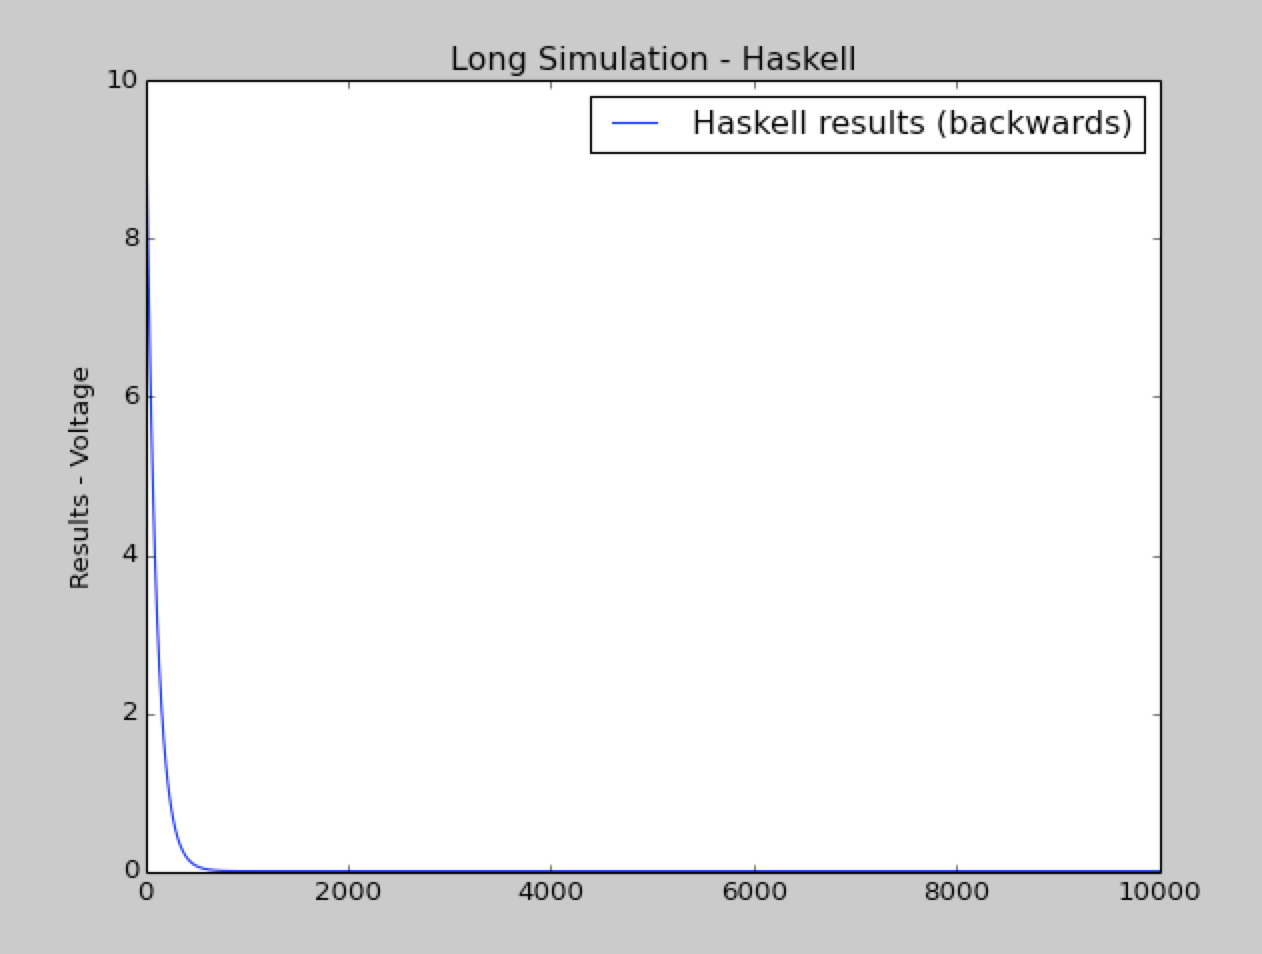
\includegraphics[width=0.7\textwidth]{img/dcresultsmicro.png}
   \caption{DC Circuit, Haskell implementation, step size of 0.000001s}
   \label{fig:dcresultsmicro}
\end{figure}

\begin{figure}[H]
   \centering
   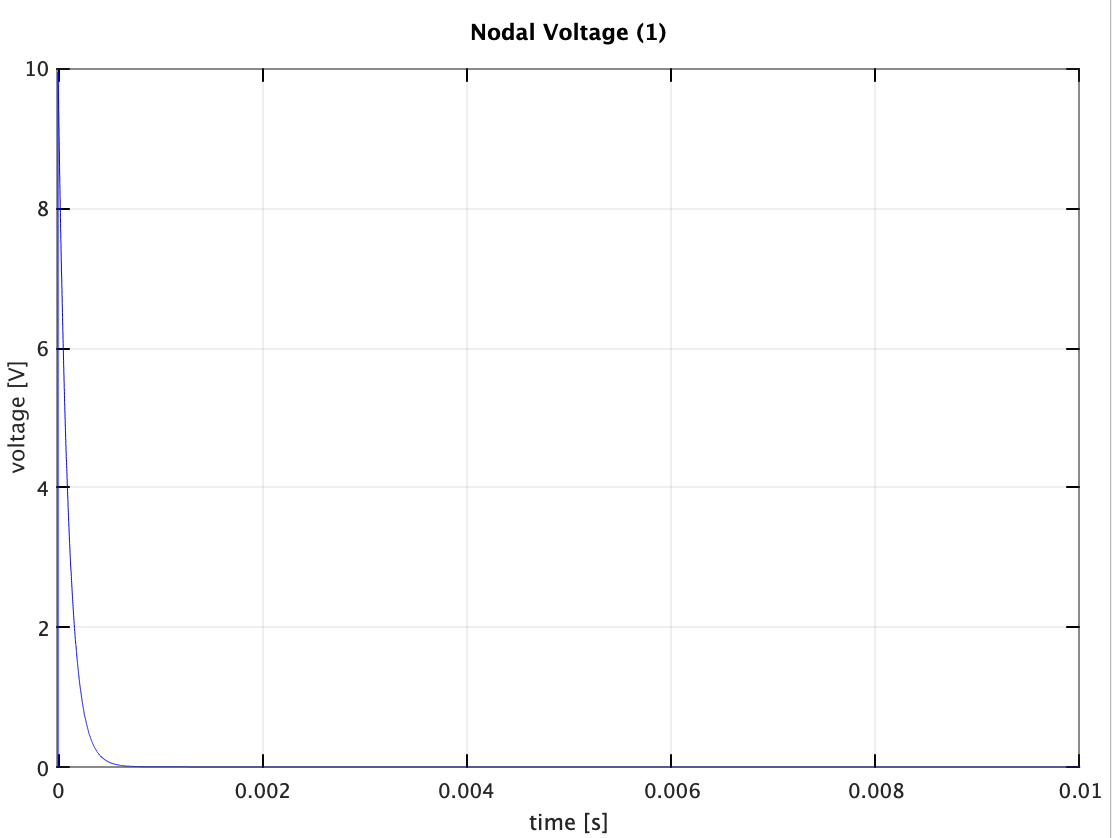
\includegraphics[width=0.7\textwidth]{img/dcresultsmicrooctave.png}
   \caption{DC Circuit, Matlab implementation, step size of 0.000001s}
   \label{fig:dcresultsmicrooctave}
\end{figure}


\subsection{Short simulation with AC Voltage}

The results for the short AC simulation (with an EAC source component) are similar for both the implementations. Listing \ref{lst:inputthtareac} is the configuration for the Matlab version, and \cref{lst:csv1reac} for the Haskell version. The circuit is described in \cref{eacresults2}.

\begin{figure}[H]
   \centering
   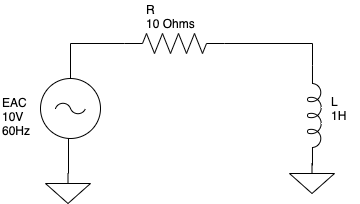
\includegraphics[width=0.7\textwidth]{img/eacresults2.png}
   \caption{AC Circuit}
   \label{eacresults2}
\end{figure}


\begin{lstlisting}[language=bash, caption={Original input data file for ETR-P Matlab}, captionpos=b, label={lst:inputthtareac}]
T   2   1   100E-6  5E-4   0   0   0   0   0
EAC 2   0   10       0      60  0   0   0   5
R   2   1   10       0      0   0   0   0   5
L   1   0   1        0      0   0   0   0   5
NV  1   2   0        0      0   0   0   0   0
\end{lstlisting}

\begin{lstlisting}[language=bash, label=getinfo, caption={Input data file for components in the Haskell implementation}, captionpos=b, label={lst:csv1reac}]
Element Type,Node K,Node M,Value,Source param 1,Source param 2,Plot
EAC,2,0,10,0,60,0
R,2,1,10,0,0,0
L,1,0,1,0,0,0
\end{lstlisting}

The results for the \lstinline!I! Vector with this configuration in Matlab are \lstinline![-970.3633e-03, 976.4595e-03]! and \lstinline![-0.9703633353209364,0.9764594717932623]! for the Haskell implementation. \ref{eacmatlab} and \ref{eachaskell} bring a comparison for the Voltage matrices in both implementations. 


\begin{figure}[H]
   \centering
   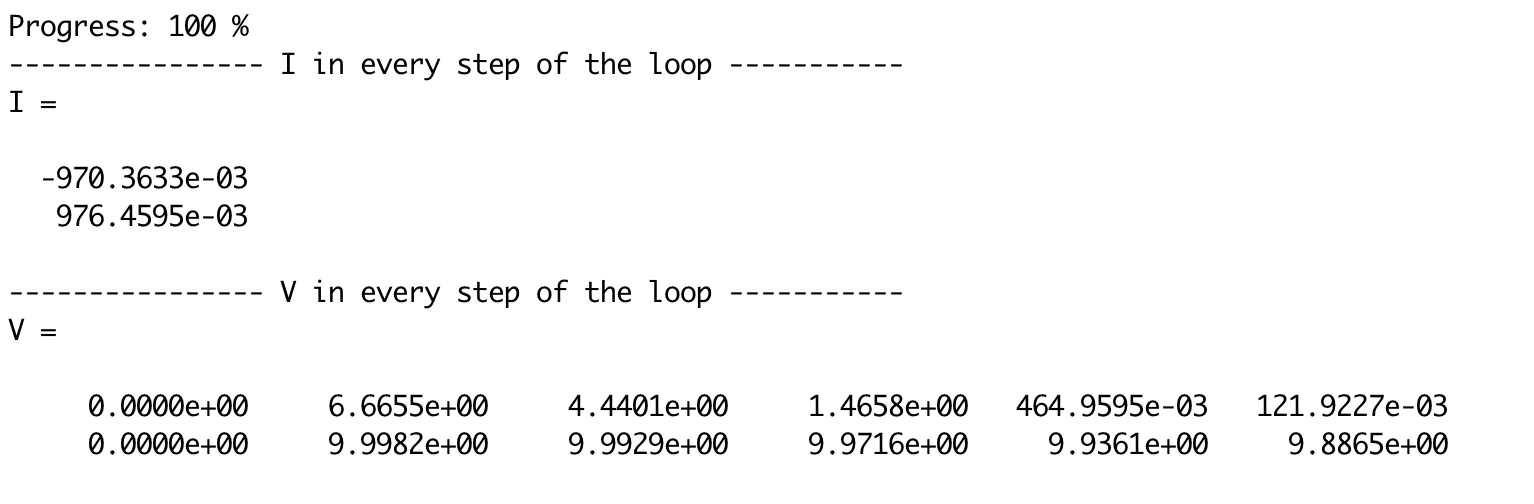
\includegraphics[width=0.7\textwidth]{img/eacmatlab.png}
   \caption{Matlab implementation - AC Voltage Source}
   \label{eacmatlab}
\end{figure}

\begin{figure}[H]
   \centering
   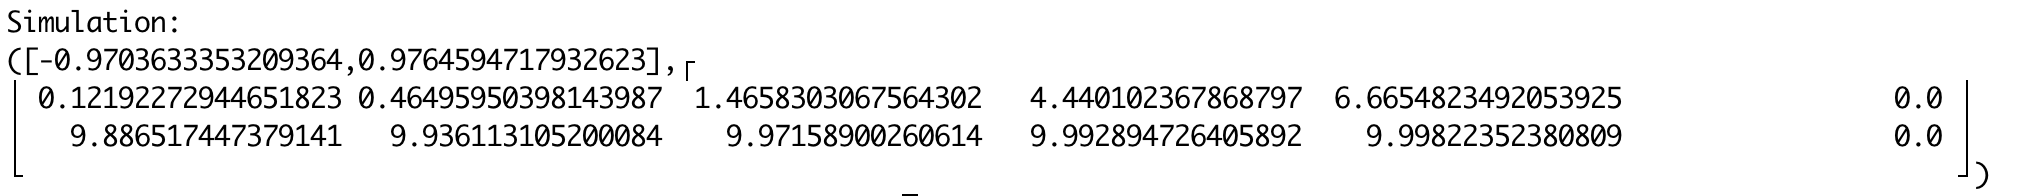
\includegraphics[width=0.7\textwidth]{img/eachaskell.png}
   \caption{Haskell implementation - AC Voltage Source}
   \label{eachaskell}
\end{figure}


\section{Simulation outputs - RC Circuit}

\subsection{Short simulation with DC Voltage}

Running a short simulation for a RC Circuit with the setup specified on \cref{lst:csv1capacitor} and \cref{lst:csv1capacitorsimulation}, it is possible to obtain the results listed on \cref{capacitorcomparison}. Once again the voltage values for the node 1 are the same in both Matlab (see \cref{capacitorcomparisonmatlab}) and Haskell (see \cref{capacitorcomparisonhaskell}) implementations. 

\begin{lstlisting}[language=bash, label=getinfo, caption={Input data file for components in the Haskell implementation}, captionpos=b, label={lst:csv1capacitor}]
Element Type,Node K,Node M,Value,Source param 1,Source param 2,Plot
EDC,2,0,10,0,60,0
R,2,1,10,0,0,0
C,1,0,1,0,0,0
\end{lstlisting}


\begin{lstlisting}[language=bash, label=getinfo, caption={Input data file for components in the Haskell implementation}, captionpos=b, label={lst:csv1capacitorsimulation}]
Number of Nodes,Number of Voltages Sources,Step Size,Maximum time for simulation
2,1,0.0001,0.0005
\end{lstlisting}

\begin{figure}[H]
   \centering
   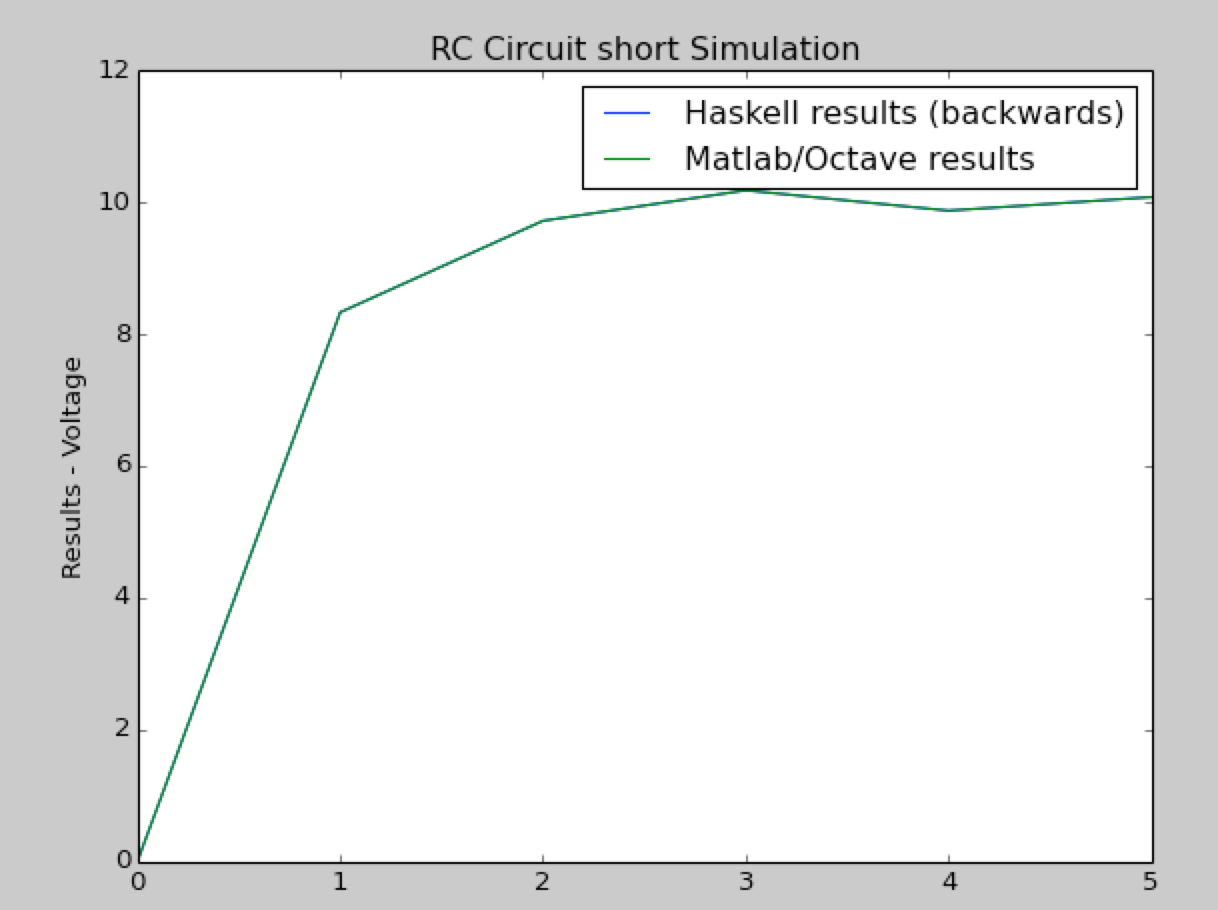
\includegraphics[width=0.7\textwidth]{img/capacitorcomparison.png}
   \caption{Comparison - DC Voltage Source for a RC Circuit}
   \label{capacitorcomparison}
\end{figure}

\begin{figure}[H]
   \centering
   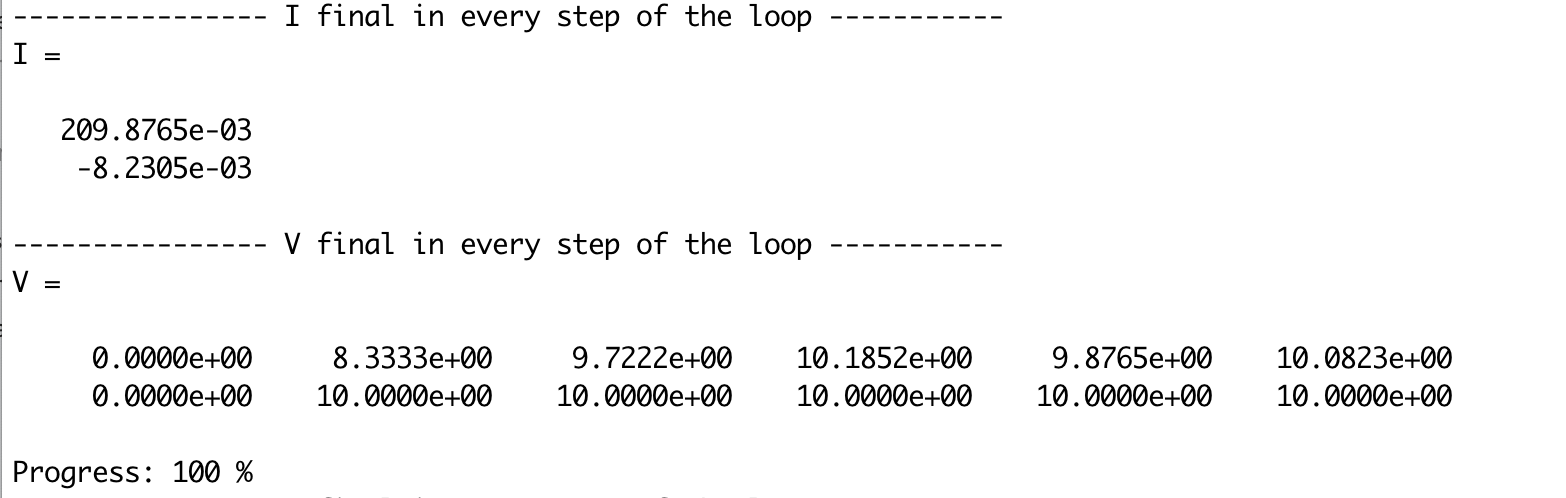
\includegraphics[width=0.7\textwidth]{img/capacitorcomparisonmatlab.png}
   \caption{Matlab results - DC Voltage Source for a RC Circuit}
   \label{capacitorcomparisonmatlab}
\end{figure}

\begin{figure}[H]
   \centering
   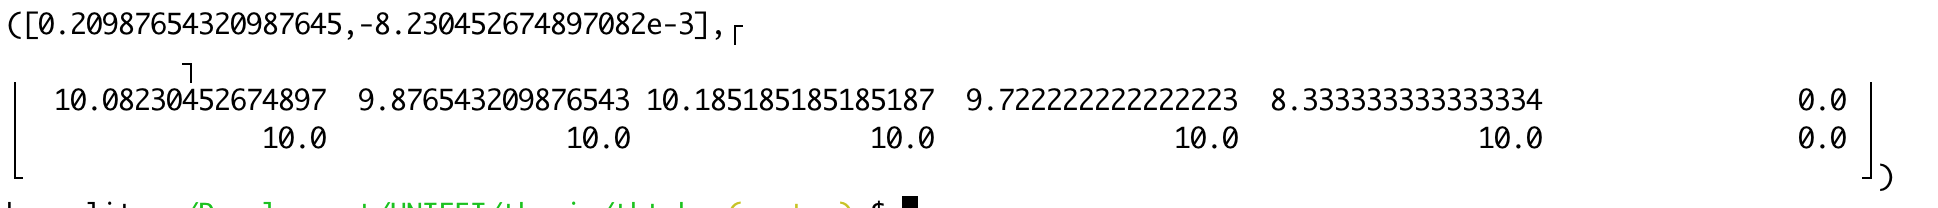
\includegraphics[width=0.7\textwidth]{img/capacitorcomparisonhaskell.png}
   \caption{Haskell results - DC Voltage Source for a RC Circuit}
   \label{capacitorcomparisonhaskell}
\end{figure}


\subsection{Short simulation with AC Voltage}

Running a short simulation for a RC Circuit with an AC source according to the setup specified on \cref{lst:csv2capacitor} and \cref{lst:csv2capacitorsimulation}, it is possible to obtain the results listed on \cref{capacitorcomparison2}. Once again the voltage values for the node 1 are the same in both Matlab (see \cref{capacitorcomparisonmatlab2}) and Haskell (see \cref{capacitorcomparisonhaskell2}) implementations. 

\begin{lstlisting}[language=bash, label=getinfo, caption={Input data file for components in the Haskell implementation}, captionpos=b, label={lst:csv2capacitor}]
Element Type,Node K,Node M,Value,Source param 1,Source param 2,Plot
EAC,2,0,10,0,60,0
R,2,1,10,0,0,0
C,1,0,1,0,0,0
\end{lstlisting}


\begin{lstlisting}[language=bash, label=getinfo, caption={Input data file for components in the Haskell implementation}, captionpos=b, label={lst:csv2capacitorsimulation}]
Number of Nodes,Number of Voltages Sources,Step Size,Maximum time for simulation
2,1,0.0001,0.0005
\end{lstlisting}

\begin{figure}[H]
   \centering
   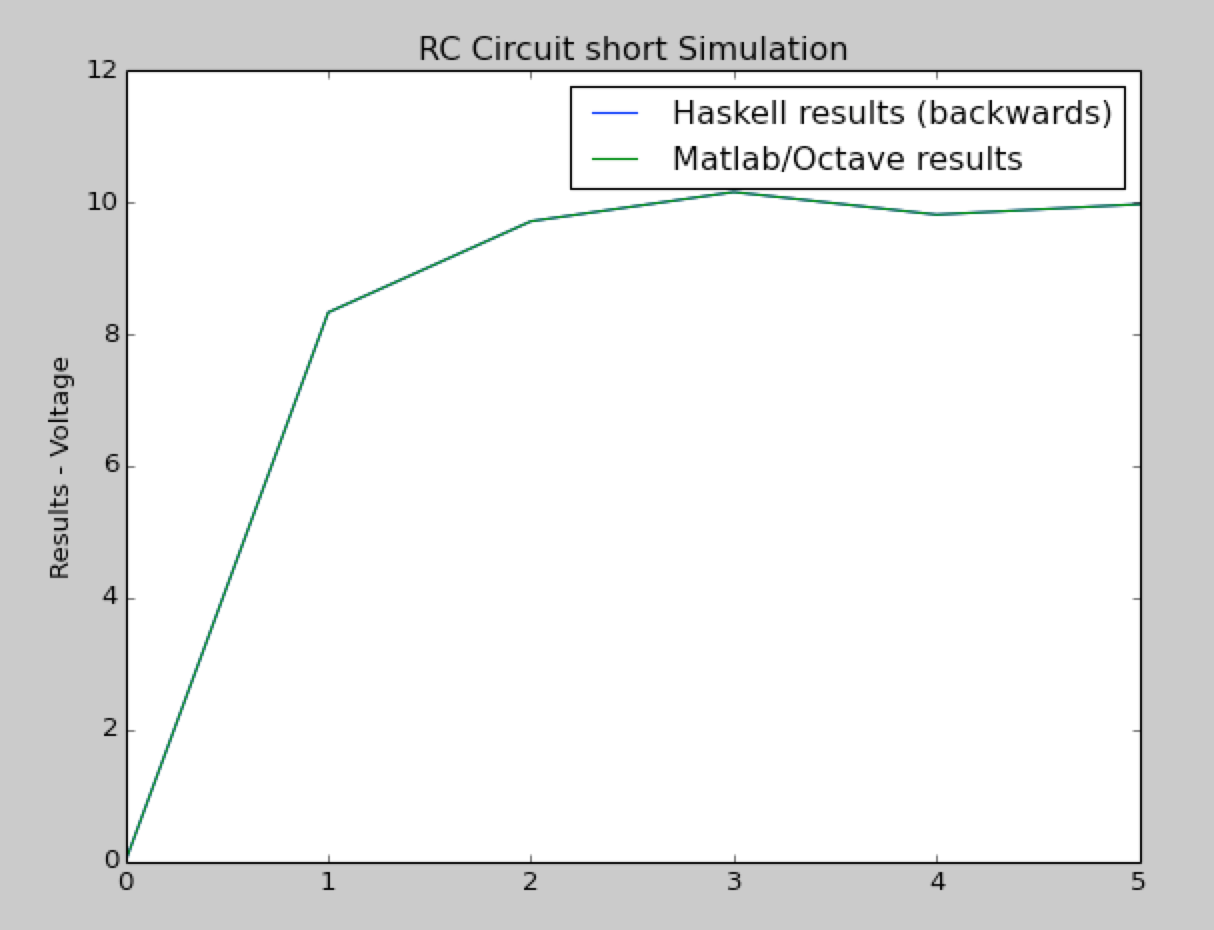
\includegraphics[width=0.7\textwidth]{img/capacitorcomparison2.png}
   \caption{Comparison - AC Voltage Source for a RC Circuit}
   \label{capacitorcomparison2}
\end{figure}

\begin{figure}[H]
   \centering
   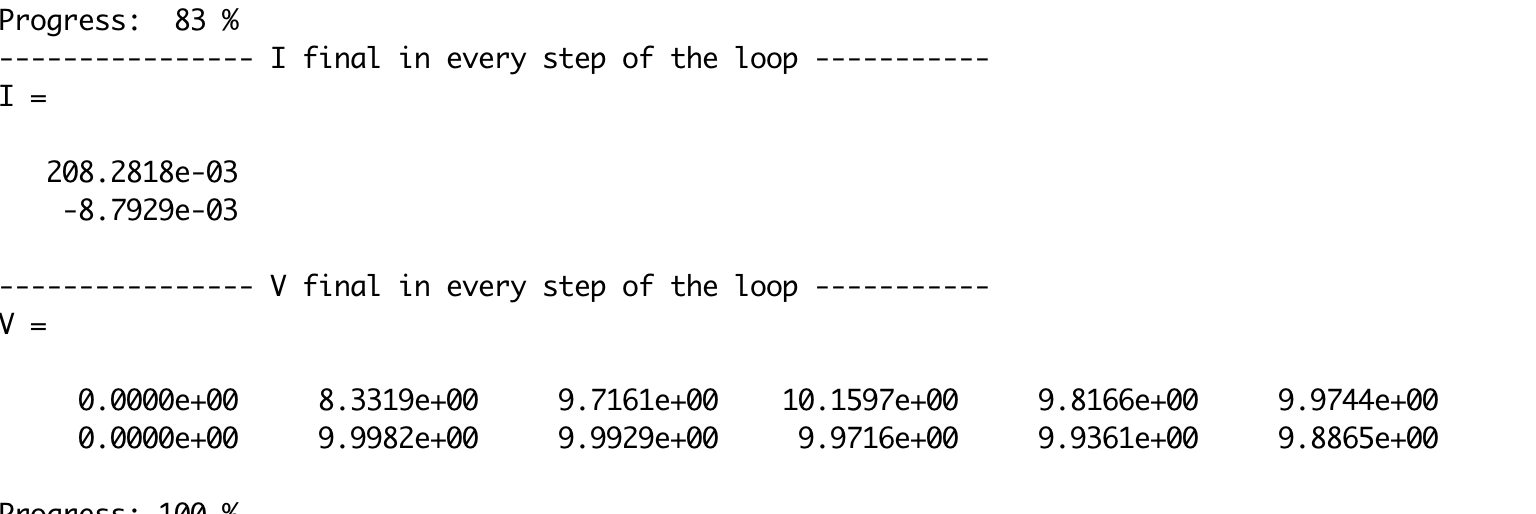
\includegraphics[width=0.7\textwidth]{img/capacitorcomparisonmatlab2.png}
   \caption{Matlab results - AC Voltage Source for a RC Circuit}
   \label{capacitorcomparisonmatlab2}
\end{figure}

\begin{figure}[H]
   \centering
   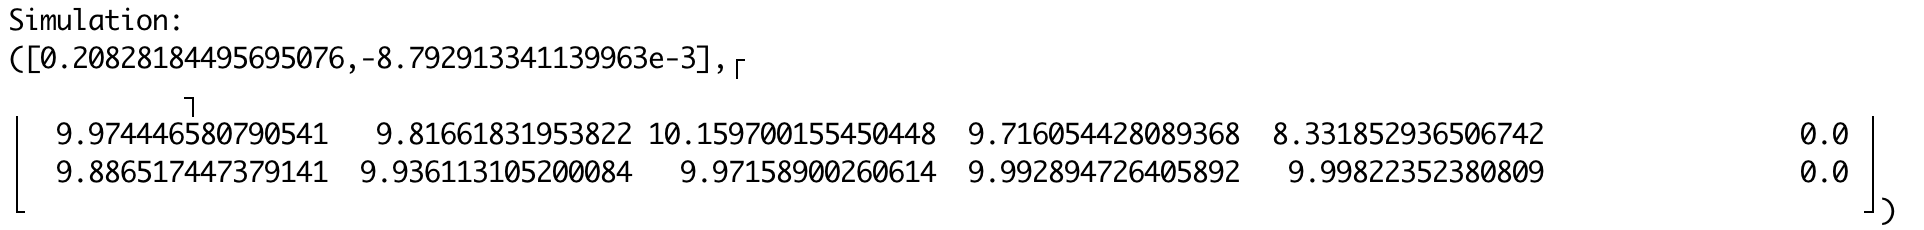
\includegraphics[width=0.7\textwidth]{img/capacitorcomparisonhaskell2.png}
   \caption{Haskell results - AC Voltage Source for a RC Circuit}
   \label{capacitorcomparisonhaskell2}
\end{figure}

\section{Recursion problems}

One of the downsides of the Haskell language was the performance of the recursive calls. Even though optimisation and execution time analysis are not the main focus of this work, it is important to mention that the overall execution time for the Haskell version of the ETR-P was slower, especially for the long simulations such as the one listed at \cref{longsimmm} for the step size of 0.000001s.


The Haskell compiler has some optimisations for dealing with recursion, such as \textit{Tail Recursion}. By building the project with special optimisation flags, it is possible to obtain slower execution times for long simulations. \lstinline!stack build --ghc-options -O2! results in longer compiler times, but in general it is possible to see a drop in the execution time. More details of other compiler flags con be found in the Haskell's GHC compiler documentation at \cite{ghc}.


\section{Using the functional approach - summary}

So far, the development of a fully functional engineering application under the functional paradigm was a challenging process especially because of the lack of references. Most of the existing implementations in the domain of electrical engineering follow the imperative style.

Choosing the appropriate types for every function was also challenging, but a careful selection guaranteed accurate results most of the time. In contrast, when developing using an imperative language, several bugs show up in runtime execution. With Haskell, most of the problems came during compile time.

Abandoning the idea of states and mutability allowed a more mathematical approach to the problem. When writing the functions, most of the time the main concern was building a meaningful and correct function chain to achieve the desired results. It was analogous to the process of developing a mathematical model to an experiment, but in the level of computer science.

The \cref{tab:funcvsimperativecod} brings a comparison between the principal differences found when writing code in both of the paradigms.

% Please add the following required packages to your document preamble:
% \usepackage{graphicx}
% \usepackage[table,xcdraw]{xcolor}
% If you use beamer only pass "xcolor=table" option, i.e. \documentclass[xcolor=table]{beamer}
\begin{table}[H]
\resizebox{\textwidth}{!}{%
\begin{tabular}{
>{\columncolor[HTML]{FFCE93}}l 
>{\columncolor[HTML]{DAE8FC}}l }
\multicolumn{1}{c}{\cellcolor[HTML]{FFCE93}\textbf{Imperative Paradigm}}      & \multicolumn{1}{c}{\cellcolor[HTML]{DAE8FC}\textbf{Functional Paradigm}}         \\ \hline
\multicolumn{1}{|l|}{\cellcolor[HTML]{FFCE93}if/else blocks}                  & \multicolumn{1}{l|}{\cellcolor[HTML]{DAE8FC}Pattern Matching}                    \\ \hline
\multicolumn{1}{|l|}{\cellcolor[HTML]{FFCE93}for and while loops}             & \multicolumn{1}{l|}{\cellcolor[HTML]{DAE8FC}Recursive calls}                     \\ \hline
\multicolumn{1}{|l|}{\cellcolor[HTML]{FFCE93}Focus on order}                  & \multicolumn{1}{l|}{\cellcolor[HTML]{DAE8FC}Focus on type}                       \\ \hline
\multicolumn{1}{|l|}{\cellcolor[HTML]{FFCE93}Most errors are runtime errors}  & \multicolumn{1}{l|}{\cellcolor[HTML]{DAE8FC}Most errors are  compile time errors} \\ \hline
\multicolumn{1}{|l|}{\cellcolor[HTML]{FFCE93}Temporary variables and binding} & \multicolumn{1}{l|}{\cellcolor[HTML]{DAE8FC}let/in construction}                 \\ \hline
\end{tabular}%
}
\caption{Code comparison: Imperative and Functional paradigms}
\label{tab:funcvsimperativecod}
\end{table}